\section{物理模型への適用と有限サンプリング実験}\label{sec:physical}
開放端横磁場イジング模型
$H=-\sum_{i=1}^NX_i-J\sum_{i=1}^{N-1}Z_iZ_{i+1}$と初期状態
$\ket+^{\otimes N}$を用いる。この模型での量子フィルタ評価は既存であり\cite{QETU}、
応用名を新規性とはしない。$N=4,6,8$、$v=(N-1)J=0.4,0.8$の6条件。
サイズとともに$J$も変わるので、熱力学的なスケーリング実験ではない。

\paragraph{対角化前に与える解析的な事前情報.}
$\Delta=2-v$、$t^2=v^2/(N-1)$、$d=t^2/\Delta$とする。
非相互作用の積状態のエネルギーは$-N$、直交ブロックは
$QHQ\succeq(-N+\Delta)Q$であり、異なる結合がX基底で異なる2スピンを反転するので
$\|QV\ket+^{\otimes N}\|^2=t^2$。基底状態を$c\ket+^{\otimes N}+q$と分けると、
変分上界$E_0\leq-N$とブロックの固有方程式から
\[
 q=-(QHQ-E_0)^{-1}QV\ket+^{\otimes N}c,\quad
 -N-E_0\leq t^2/\Delta,\quad \|q\|\leq(t/\Delta)|c|.
\]
よって$L=-N-d\leq E_0\leq U=-N$、重なり下界は
$a=1/(1+t^2/\Delta^2)$。
$R=N+v$、$G=(H-LI)/(R-L)$、$u=d/(R-L)$、$E=u/8$とする。
物理エネルギーの精度は$d/8$で、事前中点の保証誤差$d/2$より4倍厳しい。
真の固有値・重みは選択を固定した後の監査にだけ用いる。
事前境界の導出は非相互作用模型のギャップを使う。この弱結合実験で
gap-free方式の優位性を確認したとはしない。

\paragraph{Hamiltonianへの実装上の写像.}
エネルギー平均にスカラー定理を適用するため、$Y=2G-I$の理想的な正規化
Hermitian信号を仮定する。$P(x)=\sum c_kT_k(2x-1)$なら
$F(y)=P((y+1)/2)$を偶・奇部分に分け、各々をQSP合成できる。
$|F|\leq1$より各部分も$[-1,1]$で有界。安全係数0.95で合成し、
Hermitian抽出とLCU平均を使うと振幅は$0.475P(G)$となる。
追加の1/2を非自明なフィルタ候補に計上する。無フィルタ基準は抽出を省き成功確率1。
直列呼出しは高々$4n$、
準備費用は感度パラメータ$c_\psi=N$とした。実ゲート深さではない。
$Y$をPauli LCUで作る係数ノルムは$(2R+|R+L|)/(R-L)$で一般に1を超え、
正規化信号へ変換する追加操作の費用は含めない。したがって理想oracleの比較である。
$Y$の制御encodingへのHadamard testを1回行えば、結果確率は
$(1+\langle Y\rangle)/2=\langle G\rangle$となる。平方根Hamiltonianを無料で
仮定せずに、Bernoulli型energy読出しを実現する。

4スピン・$v=0.8$では積状態のバイアス0.053411が目標0.022222を超えたが、
元の次数7応答で0.000368となった。元の6応用条件すべてでバイアス目標を達成。
試したChebyshev型の保証費用は選択応答の1.001--1.173倍、認証されたpower型の
3条件では5.03--19.02倍。他の3条件は次数上限内の試した候補に認証がない。
全チューニングに対する優位性ではなく、絶対費用も大きい。
元の応用位相の連続誤差上界は最大$2.04\times10^{-16}$だが、以下では本人指定の
理想回路条件に従い目標多項式そのものを厳密とし、測定の有限性だけを加える。

\paragraph{有限予算での選択と再現.}
元の認証済み候補に、$b/u\in\{1/32,1/16,1/8,1/4,1/2\}$、
$n\in\{1,2,3,4,5,6,8,10,12,16\}$のLP候補を加える。
設計は$0.98b$、連続証明は$0.99b$で、認証に失敗した候補は除く。
無フィルタ平均も加えた6候補群の大きさは27,27,24,20,19,15。
事前中点は別の候補とする。総予算$B=10^2,10^3,\ldots,10^9$ごとに
式\eqref{eq:finite-upper}--\eqref{eq:inverse-upper}の上界を最小化し、
無出力上界を0.05以下に制限する。48条件のうち21条件では事前中点が選ばれた。
予算増加に伴い次数と誤差配分が変わる。選択には対角化の真値を使わない。

\begin{figure}[tb]
\centering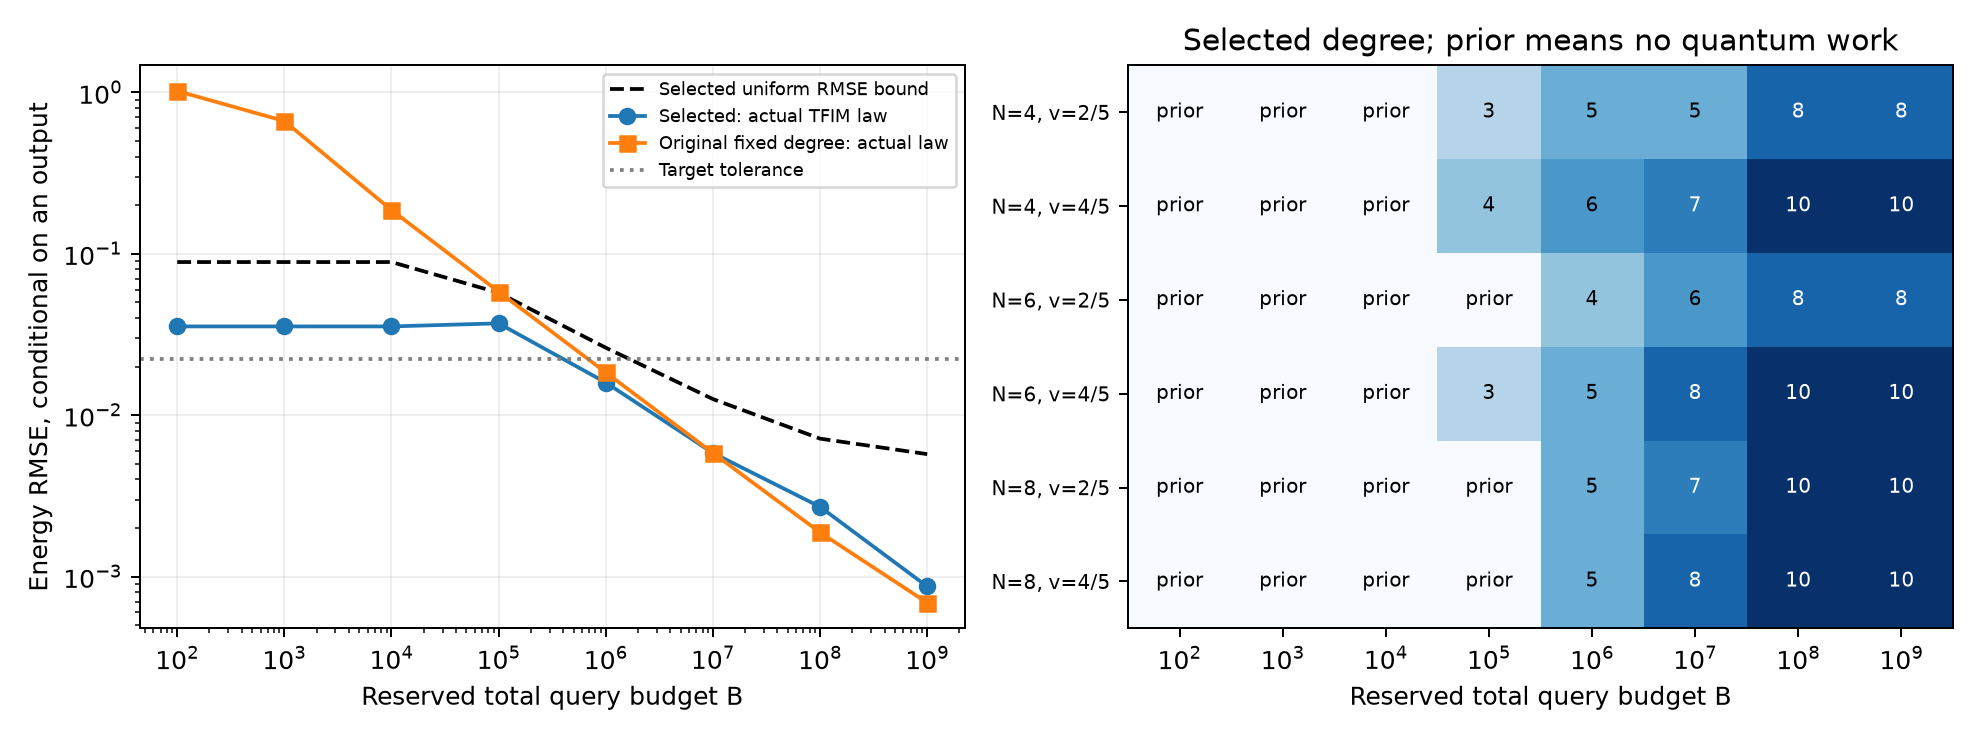
\includegraphics[width=\linewidth]{../../figures/finite_budget.png}
\caption{有限予算選択。左の黒線は一様RMSE上界、色線は4スピン・$v=0.8$での
厳密法則の数値評価。右は6事前条件で選ばれた次数。priorは量子計算なし。
一様上界の改善は各個別入力での実際のリスク改善を意味しない。}
\end{figure}

3固有値縮約は、21固有値を持つ100個の独立な入力でも検査した。
モーメントLP後は全例で支持が高々3点、平均を維持し、受理確率は増えず、
条件付きMSEも減らなかった。観測されたリスク増加は最大3.95倍。
これは証明した縮約の数値照合であり、連続最悪ケースを数値的に認証したものではない。

\paragraph{有限回の精度、信頼度、バイアスの下限.}
4スピン・$v=0.8$で元の次数7応答を固定した結果は次の通り。
\begin{center}\small
\begin{tabular}{rrrr}
\toprule
$B$ & 条件付きenergy RMSE & 無出力 & 精度違反確率\\
\midrule
$10^2$ & $1.021$ & $0.711$ & $1.000$\\
$10^6$ & $0.01840$ & $<10^{-12}$ & $0.2265$\\
$10^7$ & $0.005830$ & $<10^{-12}$ & $0.000157$\\
\bottomrule
\end{tabular}
\end{center}
$B=10^6$ではRMSEが目標0.022222より小さくても、精度違反は約22.65\%ある。
したがってRMSEだけから95\%信頼度を述べられない。
確率は式\eqref{eq:finite-failure}の二項混合を数値評価し、省略する成功数の確率は
約$10^{-12}$以下とした。正規近似ではないが、厳密有理区間証明とも区別する。

3応答を固定して$T=10^0,\ldots,10^{12}$を変えると、標本誤差の減少から
バイアスで頭打ちになる領域へ移る。次数4,7,10の物理energyバイアスはそれぞれ
0.000763、0.000368、0.000157であり、ショット数だけを増やしても消せない。
合計114バッチで各20,000回、計2,280,000回の独立集約二項サンプリングを行った。
実測MSEは厳密法則の数値値と整合し、最大の差はMonte Carlo標準誤差の3.31倍。
予算実験でランダム成功数を期待値で置き換えた予測とのMSE比は0.280--1.293だった。
別に厳密有理和・包絡演算の183チェックを通した。

\begin{figure}[tb]
\centering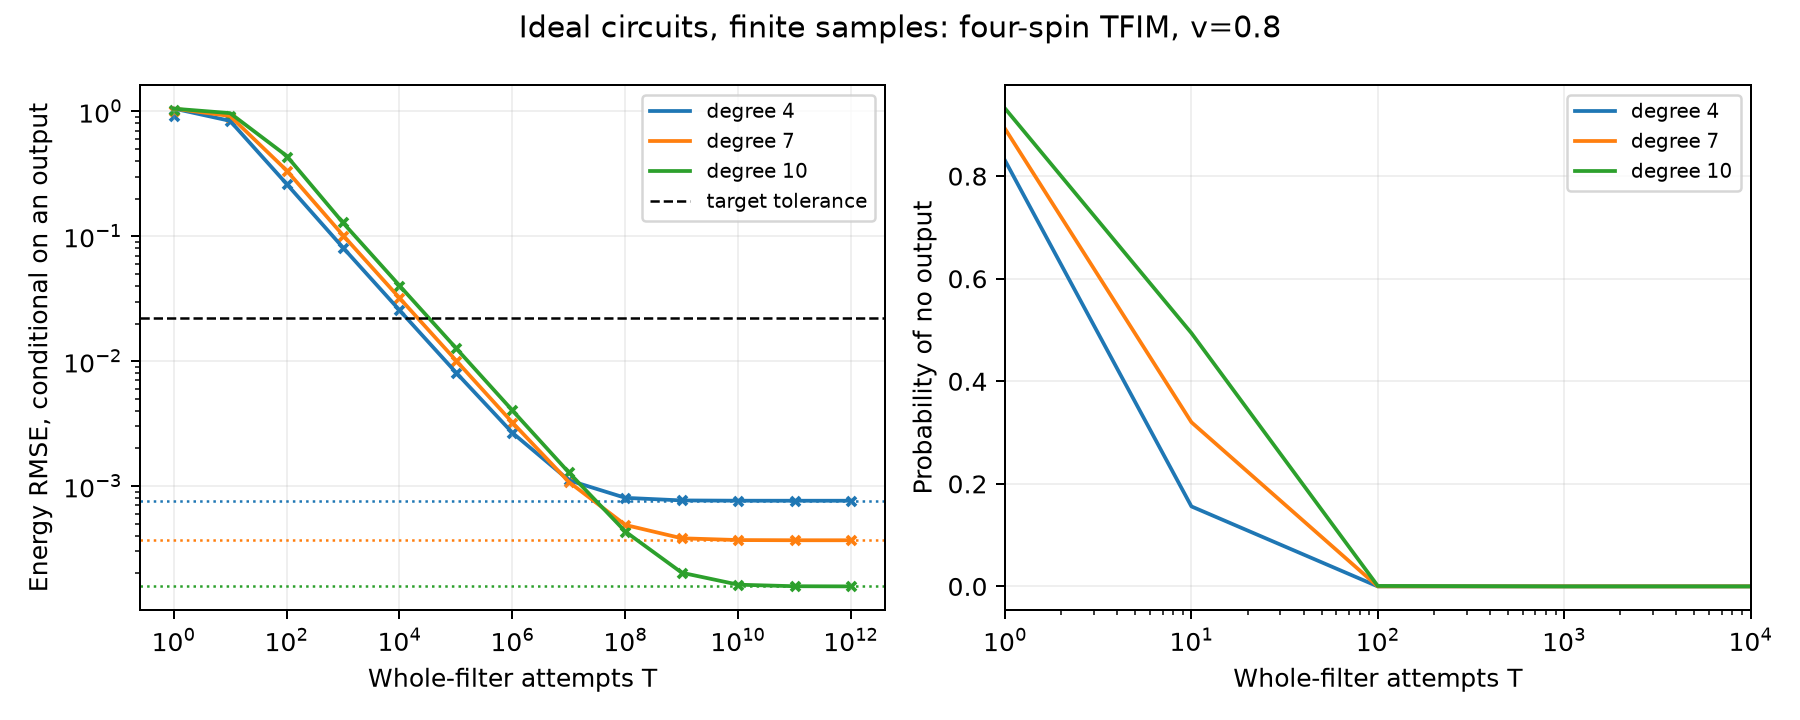
\includegraphics[width=\linewidth]{../../figures/finite_precision.png}
\caption{理想回路・有限サンプリング。線は条件付きRMSEの法則、十字はMonte Carlo、
点線はバイアス下限。右は無出力確率。目標線は許容誤差で、信頼区間の境界ではない。}
\end{figure}

頑健選択は保守的である。同じ代表例の$B=10^8$では次数10を選び、実際のRMSEは
0.00270で、元の次数7の0.00188より大きい。最小化したのは候補群内の一様保証上界で、
個別スペクトルの実リスクではない。小規模・古典的に解ける鎖なので、量子優位、
熱力学的スケーリング、QET-U等への優位性を示さない。追加の成果は、有限予算の
精度と無出力を明記した目的、スペクトル縮約、再現可能な理想サンプリング検証である。
